
\begin{frame}
    \frametitle{Типы ДЗЗ}
    Выделяют следующие типы систем:
    \begin{itemize}
        \item Пассивные: системы регистрируют отраженное от объектов солнычное излучение (оптические сканерные системы). Такие системы собычно содержат несколько каналов, каждый из которых регистрирует излучение в определенной зоне спектра.
        \item Активные: сами излучают сигнал (в области микроволнового излучения) и регистрируют вернувшийся назад отклик (радарные системы). Основное преимущество таких систем перед пассивными --- они не звисят от погоды и облачности.
    \end{itemize}
\end{frame}

\begin{frame}
    \frametitle{Излучение и атмосферные эффекты}
    \begin{figure}[!ht]
        \begin{center}
            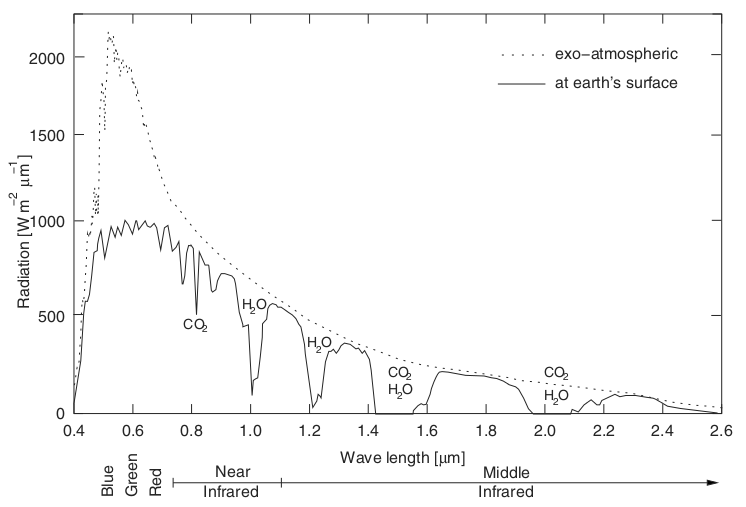
\includegraphics[width=1.0\columnwidth]{./remote_sensing/img/solar_radiation}
        \end{center}
        \caption{\tiny Neteler, Markus. Open source GIS. No. 6. SAGE Publications, 2010.}
    \end{figure}
\end{frame}
\note{
рассказать о том, как изменяется уровень излучения проходя через атмосферу. О необходимости коррекции атмосферных эффектов
}

\begin{frame}
    \frametitle{Отраженное излучение различных классов объектов}
        \begin{figure}[!ht]
        \begin{center}
            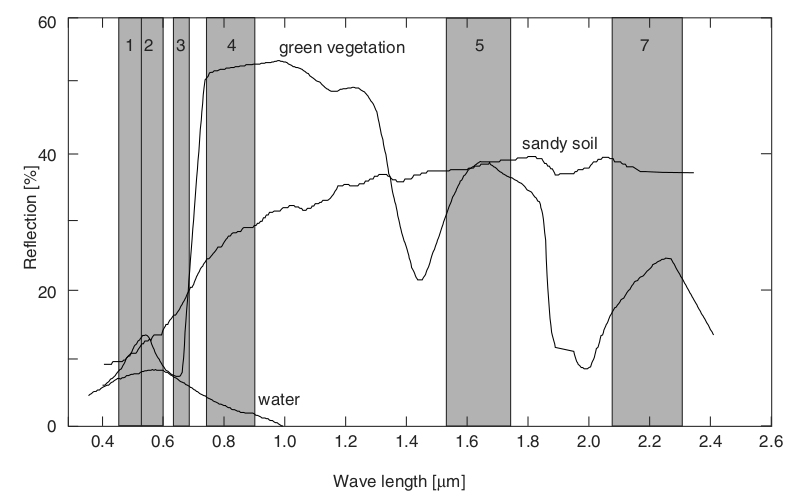
\includegraphics[width=1.0\columnwidth]{./remote_sensing/img/reflectance}
        \end{center}
        \caption{\tiny Neteler, Markus. Open source GIS. No. 6. SAGE Publications, 2010.}
    \end{figure}
\end{frame}
\note{
О том, что разные объекты отражают по разному. Что поведение линий (см. рис.) очень специфично для объектов. Что существуют специальные спектральные библиотеки.
}

\begin{frame}
    \frametitle{Данные, получаемые от оптических систем}
    Растровые изображения, характеризуются разрешением:
    \begin{itemize}
        \item пространственным;
        \item спектральным;
        \item радиометрическим.
    \end{itemize}
\end{frame}

\begin{frame}
    \frametitle{Примеры}
    \begin{figure}[!ht]
        \begin{center}
            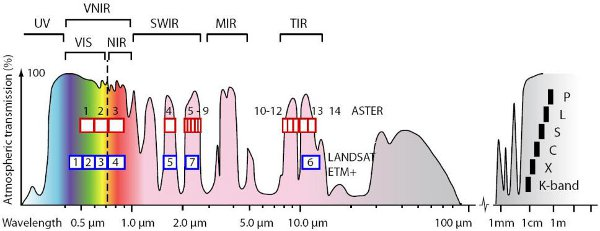
\includegraphics[width=1.0\columnwidth]{./remote_sensing/img/bands}
        \end{center}
        \caption{\tiny Kenneth A. Duda, Michael Ramsey, Rick Wessels and Jonathan Dehn (2009). Optical Satellite Volcanеo Monitoring: A Multi-Sensor Rapid Response System, Geoscience and Remote Sensing, Pei-Gee Peter Ho (Ed.)}
    \end{figure}
    Ландсат-5 : 30-метровое разрешение, однобайтовое радиометрическое разрешение.
\end{frame}

\begin{frame}
    \frametitle{Пространство признаков}
    \begin{figure}[!ht]
        \begin{center}
            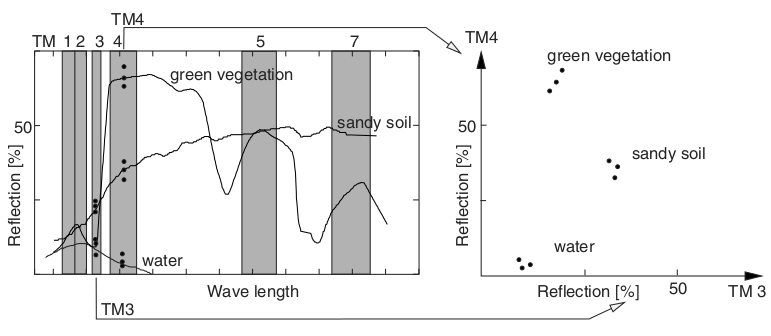
\includegraphics[width=1.0\columnwidth]{./remote_sensing/img/feature_space}
        \end{center}
        \caption{\tiny Neteler, Markus. Open source GIS. No. 6. SAGE Publications, 2010.}
    \end{figure}

\end{frame}
